\documentclass[a4paper,12pt]{report} 
\usepackage[T1]{fontenc}                                          %codifica dei font
\usepackage[utf8]{inputenc}                                     %lettere accentate da tastiera
\usepackage[english]{babel}
%lingua del documento
\usepackage{graphicx}   %inserimento immagini
\usepackage{subcaption}
\setlength\parindent{0pt}                                           %tolgo rientri a inizio paragrafo
\usepackage{titlesec}                                                 %modifica scritta capitolo
\usepackage{float}
\usepackage{geometry}                                             %serve per i margini assieme a quello sott
\usepackage[backend=biber,style=numeric,sorting=nyt]{biblatex}
\addbibresource{ref.bib}

\geometry{a4paper,top=3cm,bottom=2.5cm,left=2cm,right=2cm}  %dimensione margini
\usepackage[table,dvipsnames]{xcolor}
\usepackage{subfig}
\titleformat{\chapter}{}{}{0em}{\bfseries\LARGE\ifnum\value{chapter}>0\relax\arabic{chapter}.~\fi} %elimino scritta capitolo al loro inizio
\usepackage{titlesec}
\titlespacing*{\chapter}{0pt}{-20pt}{20pt}
\usepackage[colorlinks,citecolor=black,linkcolor=black,urlcolor=black]{hyperref}
\usepackage[font=footnotesize,labelfont=bf]{caption} 
\usepackage{hypcap}
\usepackage{wrapfig}
\usepackage{placeins}
%\titlespacing*{\chapter}{0pt}{0pt}{2pt}
\usepackage{amsmath}
\usepackage{import}
\usepackage{transparent}
\usepackage{adjustbox}
\usepackage{textcomp}
\usepackage{eurosym}
\usepackage{tikz}
\usepackage{soul}
\usetikzlibrary{tikzmark,decorations.pathreplacing}
\usepackage{pifont}
\usepackage{pdfpages}
\usepackage{appendix}
\usepackage{hyperref} %serve per inserire il link
%\newcommand{\mychapter}[2]{
%    \setcounter{chapter}{#1}
%    \setcounter{section}{0}
%    \chapter*{#2}
%    \addcontentsline{toc}{chapter}{#2}
%}

%QUESTO BLOCCO SERVE PER L'HEADING
\setlength{\headheight}{14.5pt}
\usepackage{fancyhdr}                     % get some nice header and footer options
\fancyhf{}                                % clear all header and footers
\lhead{{\slshape\nouppercase \rightmark}} %section name left side of header
\rhead{\thepage}                          %current page on right side of header
\pagestyle{fancy}
%FINO QUI PER HEADING


\begin{document}
\begin{titlepage}
\begin{center}

\begin{figure}[h]
    \begin{center}
        
\includegraphics[width=12cm]{immagini/ICARUS Nero sfondo bianco.png}
    \end{center}
\end{figure}

{\color{gray} \line(1,0){300}}\\[0.15cm]
{\Large ICARUS PoliTO - APA}\\[0.4cm]
{\bfseries \huge{HRE Design: Theory and models}}\\[0.3cm]
{\Large Version 1-00}\\
{\color{gray} \line(1,0){300}}\\

\vfill
\begin{figure}[h!]
\begin{center}

\includegraphics[width=0.5\columnwidth]{immagini/polito_black.png}
\end{center}
\end{figure}

{\Large 09 December 2025}\\[0.5cm]

\end{center}
\end{titlepage}


\newpage
\thispagestyle{empty}

\section*{Authors}
Cristian Casalanguida\\

\section*{Abstract}
To develop a Hybrid Rocket Engine it is important to possess the ability of predicting performances and costs in terms of propellant mass and volumes. To accomplish this task, different models for each component are needed.

\renewcommand{\contentsname}{Index}
\tableofcontents %genera index

\chapter{Introduction}
The main focus will be on the description of the main components needed for the engine and how they are modeled. The components are the following:
\begin{itemize}
    \item Oxidizer tank
    \item Feeding line
    \item Injector
    \item Combustion chamber
    \item Fuel grain
    \item Nozzle
\end{itemize}
Moreover, to find the best configurations, an optimization  is required.
\newpage

\newpage
\chapter{Tank}
A self-pressurizing fluid is characterized by a high vapor pressure and evaporating it can reduce the pressure drop in blow-down tanks
A tank full of oxidizer should be modeled according to the fluid properties; in particular, there are three main possible solutions:
\begin{itemize}
    \item Self-pressurizing liquid
    \item Pressurized gas
    \item Constant pressure liquid with pressurant
\end{itemize}
\section{Self-pressurizing}
A self-pressurizing model for tank blow-down is taken from \cite{Selfpress} and uses the CoolProp library in Python \cite{doi:10.1021/ie4033999}.\\
The model considers the tank to be isoentropic, considering the loss due to outflow:\\
\begin{equation}
    {s_{i+1}=\frac{s_{i}m_i-s_{L,i} \dot{m}_Ldt-s_{G,i} \dot{m}_Gdt}{m_i - \dot{m}_Ldt - \dot{m}_Gdt}}
\end{equation}
Knowing the mass and volume in every instant, it is possible to determine the total density. From density and total specific entropy we find vapor quality, pressure and temperature through the built-in fluid tables.\\

\subsection{Functions}
The functions to perform the calculations are in \textit{Tank//tank\_simulation.py}.\\
\begin{verbatim}
do_one_step(mdotL, mdotV, sL, sV, S, m, Q, oxidizer, Vtank, dt) 
-> return m_new, mL_new, mV_new, Q_new, sL_new, sV_new, S_new, ptank_new, Ttank_new
\end{verbatim}
\hspace*{2em} Performs a single step of the blow-down. Input and output description in Table \ref{Tab: StepSelf-press}.
\begin{table}[h!]
\centering
\begin{tabular}{l|l}
\hline
\textbf{Input at time \textit{i}} & \textbf{Output at time \textit{i+1}} \\
\hline
Liquid mass flow [kg/s] & Total mass [kg] \\
Vapor mass flow (through venting) [kg/s] & Liquid mass [kg] \\
Liquid specific entropy [J/(kgK)] & Vapor mass [kg] \\
Vapor specific entropy [J/(kgK)] & Vapor quality ($\frac{m_V}{m_L}$) \\
Total entropy [J/K] & Liquid specific entropy [J/(kgK)] \\
Total mass [kg] & Vapor specific entropy [J/(kgK)] \\
Vapor quality ($\frac{m_V}{m_L}$) & Total entropy [J/K] \\
Oxidizer dictionary \{"OxidizerCP": CoolProp fluid name\} & Tank pressure [Pa] \\
Tank volume [m$^3$] & Tank temperature [K] \\
Time step [s] & \\
\hline
\end{tabular}
\caption{Step function input and output for self-pressurizing tank.}
\label{Tab: StepSelf-press}
\end{table}

\begin{verbatim}
create_tank(m, Q, T, oxidizer, p=1e5)
-> return Vtank
\end{verbatim}
\hspace*{2em} Creates a self-pressurizing fluid tank: calculates each phase density and then combines them with vapor quality and total mass to get the volume. Input and output description in Table \ref{Tab: CreateSelf-press}.
\begin{table}[h!]
\centering
\begin{tabular}{l|l}
\hline
\textbf{Input at time 0} & \textbf{Output at time 0} \\
\hline
Total mass [kg] & Tank volume [m$^3$] \\
Vapor quality &  \\
Ambient temperature [K] &  \\
Oxidizer dictionary \{"OxidizerCP": CoolProp fluid name\} &  \\
\hline
\end{tabular}
\caption{create\_tank input and output for self-pressurizing tank.}
\label{Tab: CreateSelf-press}
\end{table}

\begin{verbatim}
starting_conditions(m0, T0, Vtank, oxidizer)
-> ptank0, sL0, sV0, mL0, mV0, Q0, s0, S0
\end{verbatim}
\hspace*{2em} Calculates the inputs needed for the step function at time 0. Input and output description in Table \ref{Tab: StartSelf-press}.
\begin{table}[h!]
\centering
\begin{tabular}{l|l}
\hline
\textbf{Input} & \textbf{Output} \\
\hline
Total mass [kg] & Tank pressure [Pa] \\
Ambient temperature [K] & Liquid specific entropy [J/(kgK)] \\
Tank volume [m$^3$] & Vapor specific entropy [J/(kgK)] \\
Oxidizer dictionary \{"OxidizerCP": CoolProp fluid name\} & Liquid mass [kg] \\
 & Vapor mass [kg] \\
 & Vapor quality \\
 & Total specific entropy [J/(kgK)] \\
 & Total entropy [J/K] \\
\hline
\end{tabular}
\caption{Starting conditions input and output for self-pressurizing tank.}
\label{Tab: StartSelf-press}
\end{table}
\section{Pressurized gas}
A pressurized gas in blow-down has a pressure drop without any positive effect, the strategy is to have the highest starting pressure.
\subsection{Functions}
The functions to perform the calculations are in \textit{Tank//tank\_simulation.py}.\\
They can be used without significant changes: to create the tank it is enough to insert 1 as quality and give the optional input of tank pressure.
\section{Constant pressure}
This configuration is composed of a pressure vessel, used to keep the pressure as constant as possible, and a propellant tank, pressurized at the regulation pressure to be kept.
The model is based on the self-pressurizing one, considering the system to be isoentropic. In this case the entropy is transferred from the pressure vessel to the tank ullage.
\subsection{Functions}
The functions to perform the calculations are in \textit{Tank//tank\_pressurant\_simulation.py}.\\
\begin{verbatim}
do_one_step(mdotL, mdotG, mdotpress, sL, sG, spress, mL, mG, mpress, T_tank, 
propellant, pressurant, Vtank, Vpress, dt)
-> return mL_new, mG_new, mpress_new, sL_new, sG_new,
spress_new, ptank_new, Ttank_new, p_press_new, T_press_new
\end{verbatim}
\hspace*{2em} Calculates the needed output after one time-step. Pressure is calculated using entropy and density to confirm the constant pressure behaviour. Input and output description in Table \ref{Tab: StepPressurised}.
\begin{table}[h!]
\centering
\begin{tabular}{l|l}
\hline
\textbf{Input at time \textit{i}} & \textbf{Output at time \textit{i+1}}\\
\hline
Liquid mass flow [kg/s] & Liquid mass [kg] \\
Gass mass flow (through venting and refill) [kg/s] & Gas mass [kg] \\
Pressurant mass flow (through refill) [kg/s] & Pressurant mass [kg] \\
Liquid specific entropy [J/(kgK)] & Liquid specific entropy [J/(kgK)]\\
Gas specific entropy [J/(kgK)] & Gas specific entropy [J/(kgK)]\\
Pressurant specific entropy [J/(kgK)] & Pressurant specific entropy [J/(kgK)]\\
Liquid mass [kg] & Tank pressure [Pa]\\
Gas mass [kg] & Tank temperature [K]\\
Pressurant mass [kg] & Pressure vessel pressure [Pa]\\
Tank temperature [K] & Pressure vessel temperature [K]\\
Propellant CoolProp name & \\
Pressurant CoolProp name & \\
Tank volume [m$^3$] & \\
Pressure vessel volume [m$^3$] & \\
Time step [s] & \\
\hline
\end{tabular}
\caption{Step function input and output for constant pressure tank.}
\label{Tab: StepPressurised}
\end{table}
\begin{verbatim}
create_pressurant_tank(T0, P0, V_propellant, p_reg, pressurant)
-> return V0
\end{verbatim}
\hspace*{2em} This function creates the pressure vessel considering adiabatic discharge, input and output description in Table \ref{Tab: CreatePressurised}: from \textit{First thermodynamic principle} we have
\begin{equation}
    \Delta U=U_2-U_1 =L=-pV_p
\end{equation}
with
\begin{equation*}
    U_1 = m_0c_vT_0
\end{equation*}
(values refer to pressure vessel' starting conditions)
\begin{equation*}
    U_2 = m_gc_vT_g + mc_vT
\end{equation*}
(first term refers to pressure vessel's final conditions, second to gas in the tank's final conditions)\\
With some \textit{trivial} calculations we finally obtain
\begin{equation}
    V_0=\frac{\gamma pV_p}{p_0-p_g}
\end{equation}
with
\begin{itemize}
    \item $\gamma$: specific heat ratio of the pressurant
    \item $p$: tank pressure [Pa]
    \item $V_p$: tank volume [m$^3$]
    \item $p_0$: starting vessel pressure [Pa]
    \item $p_g$: final vessel pressure, assumed $1.2p$ [Pa]
\end{itemize}

\begin{table}[h!]
\centering
\begin{tabular}{l|l}
\hline
\textbf{Input} & \textbf{Output}\\
\hline
Ambient temperature [K] & Pressure vessel volume [m$^3$]\\
Vessel pressure [Pa] & \\
Propellant volume [m$^3$] & \\
Tank pressure [Pa] & \\
Pressurant CoolProp name & \\
\hline
\end{tabular}
\caption{create\_pressurant\_tank input and output for constant pressure tank.}
\label{Tab: CreatePressurised}
\end{table}

\begin{verbatim}
create_propellant_tank(mp0, p0, T0, Q0, propellant, pressurant)
-> return V_tank, V_liq
\end{verbatim}
\hspace*{2em} Calculates the tank volume and liquid volume with a given ullage of pressurant (assumes the liquid is kept above vapor pressure). Input and output description in Table \ref{Tab: CreateProp}.
\begin{table}[h!]
\centering
\begin{tabular}{l|l}
\hline
\textbf{Input} & \textbf{Output}\\
\hline
Propellant mass [kg] & Tank volume [m$^3$]\\
Tank pressure [Pa] & Liquid volume [m$^3$]\\
Ambient temperature [K] & \\
Vapor quality & \\
Propellant CoolProp name & \\
Pressurant CoolProp name & \\
\hline
\end{tabular}
\caption{create\_propellant\_tank input and output for constant pressure tank.}
\label{Tab: CreateProp}
\end{table}

\begin{verbatim}
starting_conditions(mL, T, ptank, ppress, Vtank, Vpress, propellant, pressurant)
->return sL, sG, spress, mG, mpress
\end{verbatim}
\hspace*{2em} Calculates the needed input for the step function. Input and output description in Table \ref{Tab: StartingPress}.
\begin{table}[h!]
\centering
\begin{tabular}{l|l}
\hline
\textbf{Input at time 0} & \textbf{Output at time 0}\\
\hline
Propellant mass [kg] & Liquid specific entropy [J/(kgK)] \\
Ambient temperature [K] & Ullage gas specific entropy [J/(kgK)] \\
Tank pressure [Pa] & Pressurant specific entropy [J/(kgK)]\\
Vessel pressure [Pa] & Ullage mass [kg]\\
Tank volume [m$^3$] & Pressurant mass [kg]\\
Pressure vessel volume [m$^3$] & \\
Propellant CoolProp name & \\
Pressurant CoolProp name & \\
\hline
\end{tabular}
\caption{starting\_condition input and output for constant pressure tank.}
\label{Tab: StartingPress}
\end{table}

\section{Wrapper}
To use one of the three possible tank configurations a series of wrap functions are available in \textit{Tank//tank\_update.py}.
\begin{verbatim}
build_tank(m, Q, T, oxidizer, pressurant=None, ppress=1e5, p=1e5, plim=None)
-> return masses, volumes, pressures, temperatures, constant_pressure_tank
\end{verbatim}
\hspace*{2em} Chooses which function should be used to build the tank. To begin it tries to get the vapor pressure, if it cannot the fluid is super-critic at the given temperature, so it will be full gas (vapor quality overwritten to 1).
If it is full gas, it lowers the pressure at vapor pressure if it's higher to avoid liquid formation.
If quality is lower than 1 (liquid phase is present) and pressure is higher than vapor pressure, it is a constant pressure tank (flag set as True), else it is self-pressurized or full gas.

\begin{verbatim}
start_conditions(masses, volumes, pressures, temperatures,
oxidizer, pressurant=None, constant_pressure_tank = False)
-> return ptank, Ttank, mL, entropies_out, masses_out,
pressures_out, temperatures_out
\end{verbatim}
\hspace*{2em} Based on the \verb|constant\_pressure\_tank| flag, it selects the needed starting conditions function.

\begin{verbatim}
update_tank(mdotL, dt, entropies, masses, volumes, pressures, temperatures,
utilities, oxidizer, pressurant=None, constant_pressure_tank = False)
-> return ptank_new, Ttank_new, mL_new, entropies_out, masses_out, pressures_out, temperatures_out
\end{verbatim}
\hspace*{2em} Performs one time-step based on the \verb|constant\_pressure\_tank| flag.\\
It should be noticed that, to avoid excessive input and output and hard-to-understand variables, it was chosen to use helper dictionaries for every type of property. They vary with the type of tank and are described in Table \ref{Tab: TankDicts}\\
\begin{table}[h!]
\centering
\resizebox{\textwidth}{!}{
\begin{tabular}{l|l|l}
\hline
& \textbf{Constant pressure} & \textbf{Full gas or self-pressurizing}\\
\hline

masses & Liquid mass "mL" [kg] & Total mass "m" [kg]\\
& Gas mass "mG" [kg] & Vapor quality "Q"\\
& Pressurant mass "mpress" [kg] & Liquid mass "mL" [kg]\\
& Vent outflow "mdot\_vent" [kg/s] & Vapor mass "mG" [kg]\\
& & Vent outflow "mdot\_vent" [kg/s]\\
\hline
entropies & Liquid specific entropy "sL" [J/(kgK)] & Liquid specific entropy "sL" [J/(kgK)]\\
& Gas specific entropy "sG" [J/(kgK)] & Vapor specific entropy "sG" [J/(kgK)]\\
& Pressurant specific entropy "spress" [J/(kgK)] & Total entropy "S" [J/K]\\
\hline
pressures & Vessel pressure "ppress" [Pa] & Tank pressure "ptank" [Pa]\\
& Tank pressure "ptank" [Pa] & Tank limit pressure "plim" [Pa]\\
& Tank limit pressure "plim" [Pa] & \\
\hline
temperatures & Pressurant temperature "Tpress" [K] & Tank temperature "Ttank" [K]\\
& Tank temperature "Ttank" [K] & \\
\hline
volumes & Tank volume "Vtank" [m$^3$] & Tank volume "Vtank" [m$^3$]\\
& Pressure vessel volume "Vpress" [m$^3$] & \\
\hline
utilities & Pressurant line discharge coefficient "CDpress" & Venting valve discharge coefficient "CDvent"\\
& Pressurant line injection area "Apress" [m$^2$] & Venting valve outlet area "Avent" [m$^2$]\\
& Venting valve discharge coefficient "CDvent" & \\
& Venting valve outlet area "Avent" [m$^2$] & \\
\hline
\end{tabular}
}
\caption{Helper dictionaries keys and values for different tank configurations.}
\label{Tab: TankDicts}
\end{table}

A final consideration is that this kind of wrapping allows for a fouth kind of tank, a pressurised liquid in blow-down from a given pressure. The simple trick is to consider a pressurant line injection area equal to 0.
This configuration is meant to allow an easy implementation of the same functions in case of a \textit{bi-liquid propellant engine}.

\newpage
\chapter{Feeding line}
The purpose of the functions is to calculate with higher accuracy the injection pressure using a loss model of the feeding line.

\newpage
\chapter{Injection}
The purpose of the following models is to describe accurately the mass flow injection in different conditions.
As for the tank, the type of fluid influences the model to be used: to match the characteristics of a self-pressurising fluid
the Non-Homogeneus Non-Equilibrium (NHNE) model \cite{MassFlowRate2013} was used.
It basically condiders a weighted average of the Homogeneus Equilibrium Model,
with no slip and multi-phase fluid
\begin{equation}
	\dot{m}_{HEM}=A\rho \sqrt{2(h_1-h_2)}
\end{equation}
and the Single Phase Injection
\begin{equation}
	\dot{m}_{SPI}=A \sqrt{2\rho (p_1-p_2)}
\end{equation}
The weight takes into account the pressure drop and the drop respect to the vapor pressure
\begin{equation}
	\chi=\sqrt{\frac{p_1-p_2}{p_V-p_2}}
\end{equation}
and finally the mass flow can be calculated as
\begin{equation}
	\dot{m}_{NHNE}=\frac{\chi}{\chi+1}\dot{m}_{SPI}+\frac{1}{\chi+1}\dot{m}_{HEM}
\end{equation}
This model clearly applies to liquid or multi-phase flow, instead with an ideal gas we write
\begin{equation}
	\dot{m}_{gas}= \frac{p_1A}{\sqrt{RT_1}}f(\frac{p_2}{p_1})
\end{equation}
with
\begin{equation*}
	f(\frac{p_2}{p_1})=\sqrt{\frac{2\gamma}{\gamma -1}((\frac{p_2}{p_1})^\frac{2}{\gamma}-(\frac{p_2}{p_1})^\frac{\gamma +1}{\gamma})}
\end{equation*}
remembering that a chocked exit section is reached when
\begin{equation}
	\frac{p_2}{p_1} \leq (\frac{p_e}{p_1})_{crit}=(\frac{2}{\gamma +1})^\frac{\gamma}{\gamma -1}
\end{equation}
and in that case we write
\begin{equation}
	\dot{m}_{gas}= \frac{p_1A}{\sqrt{RT_1}}\Gamma
\end{equation}
with
\begin{equation*}
	\Gamma=\sqrt{\gamma (\frac{2}{\gamma +1})^\frac{\gamma +1}{\gamma -1}}
\end{equation*}
\section{Functions}
The following functions are in \textit{Injection//PyInjection.py}.
\begin{verbatim}
NHNE_injection(p1, p2, T, cD, fluid)
-> return mdot
\end{verbatim}
\hspace{2em} Calculates mass flux [kg/sm$^2$] using NHNE model.
Returns $0$ if $p_1<p_2$.
 \begin{verbatim}
gas_injection(p1, p2, T, CD, fluid)
-> return mdot
\end{verbatim}
\hspace{2em} Calculates mass flux [kg/sm$^2$] for an ideal gas using CoolProp properties.
Returns $0$ if $p_1<p_2$.
\begin{verbatim}
gas_injection_custom(p1, p2, T, CD, gamma, M, eps=1.0)
-> return mdot
\end{verbatim}
\hspace{2em} Calculates mass flux [kg/sm$^2$] for an ideal gas.
It is meant to be used for nozzle outflow, using burned gas properties, 
so it takes in input also the expansion ratio,modifying the chocked condition to
\begin{equation}
	f(\frac{p_2}{p_1}) \geq \frac{\Gamma}{\varepsilon}
\end{equation}
Returns $0$ if $p_1<p_2$.
\begin{verbatim}
massflow(p1, p2, T, CD, fluid)
-> return mdot
\end{verbatim}
\hspace{2em} Chooses the model to use with a \textit{try/except} structure, because the calculation of vapor pressure using CoolProp will
fail if it is super-critical.\\

All the previous functions take into account the effects of the discharge coefficient.






\newpage
\chapter{Performance}
The purpose of this function is to calculate the performances for a certain condition and handle the needed calculations for the following functions.
The calculation is based on the following assumptions: 
\begin{itemize}
	\item the combustion is in chemical equilibrium
	\item infinite area combustor
	\item frozen equilibrium at throat section
\end{itemize}
To perform this calculations NASA CEA \cite{NASACEA} and its Python wrapper
RocketCEA \cite{RocketCEA} were used.
\section{Functions}
The following functions are available in \texit{Performance//performance\_singlepoint.py}.
\begin{verbatim}
calculate_performance(Ainj, Aport, Ab, eps, ptank, Ttank, pc, CD,
                          a, n, rho_fuel, oxidizer, fuel, pamb=0.0, gamma0=1.3)
-> return (p_inj, mdot_ox, mdot_fuel, mdot, Gox, r, MR, Tc, MW, gamma, eps_out, cs,
            CF_vac, CF, Ivac, Is, flag_performance)
\end{verbatim}
\hspace{2em} Calculates the line losses and the injected mass flow, uses it to get oxidizer mass flux for the regression rate
\begin{equation}
	r=aG_{ox}^n
\end{equation}
to calculate the fuel mass flow
\begin{equation}
	\dot{m}_{fuel}=\rho_f A_b r
\end{equation}
from it the mixture ratio can be calculated as
\begin{equation}
	MR=\frac{\dot{m}_{ox}}{\dot{m}_{f}}
\end{equation}
With that we have the three needed inputs for the CEA calculations (chamber pressure, mixture ratio and expansion ratio).\\
It is possible to ask for the adapted expansion ratio passing \verb|eps="adapt"|, and it will be calculated as
\begin{equation}
	\varepsilon = \frac{\Gamma}{f(\frac{p_{amb}}{p_c})}
\end{equation}
with
\begin{align*}
	\Gamma&=\sqrt{\gamma (\frac{2}{\gamma +1})^\frac{\gamma +1}{\gamma -1}}\\
	f(\frac{p_{amb}}{p_1})&=\sqrt{\frac{2\gamma}{\gamma -1}((\frac{p_{amb}}{p_1})^\frac{2}{\gamma}-(\frac{p_{amb}}{p_1})^\frac{\gamma +1}{\gamma})}
\end{align*}

\begin{verbatim}
pressure_fun(Ainj, Aport, At, Ab, eps, ptank, Ttank, pc, CD, a, n, rho_fuel, 
			oxidizer, fuel, pamb=0.0, gamma0=1.3)
-> return Fpc
\end{verbatim}
\hspace{2em} From the definition
\begin{equation}
	c^*=\frac{p_cA_t}{\dot{m}}
\end{equation}
and we use it to calculate the pressure function to find the steady state pressure
for the optimisation:
\begin{equation}
	F(p_c)=\frac{\dot{m}c^*}{A_t} - pc
	\label{eq:PressFunction}
\end{equation}








\newpage
\chapter{Optimisation}
The purpose of these functions is to find the best configuration for a certain fuel/oxidizer combination.
\newpage
\chapter{Grain geometry}
The purpose of these functions is to give the possibility to manage complex and helical geometries, their evolution through combustion and to perform needed calculations.

\section{Calculation functions}
To perform the needed operations the following functions were built, available in \textit{Geometry//geometry\_calculation.py}.

\begin{verbatim}
create_regular_poligon(n_sides, circum_radius)
-> return x_poly, y_poly
\end{verbatim}

\hspace*{2em} Creates a centered, regular polygon inscribed in the circumference. Returns Numpy \cite{harris2020array} arrays of size $(n,)$ composed of x and y values of the vertices.

\begin{verbatim}
create_repeated_instance(x, y, n_instances)
-> return x_u, y_u
\end{verbatim}
\hspace*{2em} Given an instance of points as two Numpy arrays of size $(n,)$, repeats it \textit{n\_instances} times. Points sharing the same position are filtered returning only uniques. Returns Numpy arrays of size $(n,)$ composed of x and y values of the figure.

\begin{verbatim}
translate_figure(x, y)
-> return x_translated, y_translated
\end{verbatim}
\hspace*{2em} Positions the origin in the figure's centroid. Returns Numpy arrays of size $(n,)$ composed of x and y values of the translated figure.

\begin{verbatim}
sort_input(x, y, z=1)
-> return x_sorted, y_sorted
\end{verbatim}
\hspace*{2em} Sorts the points in counter-clockwise order if \verb|z=1| or clockwise if \verb|z=-1|, with \textit{z} rotation axis' versor. Returns Numpy arrays of size $(n,)$ composed of sorted x and y values of the figure.

\begin{verbatim}
fill_borders(x, y, n_points_per_side)
-> return x_fill, y_fill
\end{verbatim}
\hspace*{2em} Fills the segment between each consecutive point with input number of points. Returns Numpy arrays of size $(n,)$ composed of x and y values of the figure.

\begin{verbatim}
fill_borders_circumference(x, y, n_points_per_side)
-> return x_fill, y_fill
\end{verbatim}
\hspace*{2em} Fills between every consecutive point at the same radius with an arc of angle-wise linearly spaced points with the same radius. In other cases fills the segments. Returns Numpy arrays of size $(n,)$ composed of x and y values of the figure.

\begin{verbatim}
calculate_surfaces_from_points(x, y, lc, step=0.0)
-> return PortArea, BurningArea
\end{verbatim}
\hspace*{2em} Calculates the base and side area of a parallelepipedon with base given by \verb|x,y| points and height equal to \verb|lc|. It is possible to consider a twisted body giving a non-zero value to \verb|step|, which is the axial distance during a $360°$ turn. The function closes the polygon (it is not needed to repeat the first point), calculates the module of every side (linear approximation of circumferences: it should be used with filled geometries) and the radius of each vertex.\\ 
The port (base) area is calculated as the sum of each triangle's area (radius-side-radius) using Heron of Alexandria's formula:
\begin{equation}
    A = \sqrt{p\cdot(p-a)\cdot(p-b)\cdot(p-c)}
\end{equation}
with:
\begin{itemize}
    \item $p$: half-perimeter of the triangle
    \item $a, b, c$: sides of the triangle
\end{itemize}
\hspace*{2em} The side area is calculated as
\begin{equation}
    A=2p \cdot l_c
\end{equation}
for not twisted bodies. Instead with twisted bodies we divide the height in small units
\begin{equation}
    h=min(min(c), step) / 10
\end{equation}
with $c$ sides of the figure, rotate each point of the rotation at that height
\begin{equation}
    d\theta=2\pi\frac{h}{step}
\end{equation}
Then we get the distance between each translated point and the starting side with Pythagoras' theorem using height $h$ and the distance between the projection of the translated point (T) on the base plane and a straight line formed by the original point (A) and its following (B):
\begin{equation}
    H=\sqrt{h^2 + s^2}
\end{equation}
with
\begin{equation*}
    s = \frac{|(x_B-x_A)(y_T-y_A) - (y_B-y_A)(x_T-x_A)|}{\sqrt{(y_B-y_A)^2 + (x_B-x_A)^2}}
\end{equation*}
Finally, we find the area of each parallelogram, sum them and multiply by the number of height sections
\begin{equation}
    A=\frac{l_c}{h} \sum{H\cdot c}
\end{equation}

\begin{verbatim}
fill_and_calculate_surfaces_and_volume(x, y, lc, n_pointsperside=20, 
circular=False, step=0.0, Vol_prechamber=0.0, Vol_postchamber=0.0)
-> return A_port, A_burn, Vol_chamber
\end{verbatim}
This function wraps the previous, filling the borders using the self-evident flag \verb|circular| to know which function choose, calculates port area and burning area and calculates the internal fluid volume of the chamber as
\begin{equation}
    V = V_{pre} + A_pl_c + V_{post} 
\end{equation}
allowing to consider the effects of pre-chamber and mixer.\\
The main reason of this function is to have an easy call for the needed calculation considering that to update the geometry the linear and circular fills are removed to burn the actual sides without errors, as it will be later discussed.

\begin{verbatim}
calculate_fuel_mass(Ap, lc, D_chamber, fuel_density)
-> return mfuel
\end{verbatim}
\hspace*{2em} Calculates fuel mass as
\begin{equation}
    m_{fuel}=\rho_{fuel}(\frac{\pi}{4}D_{chamber}^2 - A_p)l_c
\end{equation}

\section{Update functions}
To update the geometry through the combustion process the following functions were built, available in \textit{Geometry//geometry_update.py}. 
\begin{verbatim}
remove_close_vertices(x, y, tol=1e-12)
-> return pts2[:, 0], pts2[:, 1]
\end{verbatim}
\hspace*{2em} Removes points closer than the tolerance \verb|tol| respect to the ones before. Returns Numpy arrays of size $(n,)$ composed of non-close x and y values of the figure.

\begin{verbatim}
remove_collinear_simple(x, y, tol=1e-12)
-> return x_new, y_new
\end{verbatim}
\hspace*{2em} Removes a point if it is collinear with the one before and the one after.  Returns Numpy arrays of size $(n,)$ composed of x and y vertex of the figure.

\begin{verbatim}
remove_samearc_simple(x, y, tol=1e-12)
-> return x_new, y_new
\end{verbatim}
\hspace*{2em} Removes a point if it is at the same radius of the one before and the one after.  Returns Numpy arrays of size $(n,)$ composed of non-circumferential x and y of the figure.

\begin{verbatim}
_line_intersection_from_dirs(pA, vA, pB, vB, eps=1e-12)
-> return bool, pt, s, t, cond
\end{verbatim}
\hspace*{2em} Solves a linear system to find the intersection between two lines starting from point A and B knowing the directions. Returns a flag to know if the solution was found, the intersection point, the distances from the two points and the condition number. Considering that the two directions are towards the expected intersection, distances \verb|s| and \verb|t| should be positive.

\begin{verbatim}
burn_surface(x, y, z, regression_rate, dt, min_param=1e-9, 
parallel_dot_thresh=0.9999, close_tol=1e-12, merge_tol=1e-9)
-> return x_new, y_new
\end{verbatim}
\hspace*{2em} Removes collinear points to isolate the vertex, finds the direction between each point and it's following. \verb|z| represents the rotation axis for the order of the points ($1$ if couter-clockwise and $-1$ if clock-wise) and is needed to find the normal direction for burning, in fact for counter-clockwise order we have
\begin{equation}
    t=(t_x,t_y)
\end{equation}
\begin{equation}
    n=(t_y,-t_x)
\end{equation}
and for clock-wise, instead
\begin{equation}
    n=(-t_y,t_x)
\end{equation}
So we can write
\begin{equation}
    n=(zt_y,-zt_x)
\end{equation}
We finally find the middle points of each segment and translate it of a vector
\begin{equation}
    r_n=rdt(zt_y,-zt_x)
\end{equation}
To find the intersections it is necessary to discern between sides with obtuse and acute angles, calculated using the cross product of the two normals
\begin{gather}
    z(n_A \times n_B)= \begin{matrix} >1 & obtuse\ angle\\ <1& acute\ angle\end{matrix}
\end{gather}
For obtuse angles it is enough to do the intersection, instead with acute angles we have a cusp and need to know if it does not degenerate. It happens when the cusp becomes a single side and could degenerate changing the position of two following translated mid-points. This condition is verified when the side of one of the two sides is lower than the critical distance
\begin{equation}
    L_{crit}=\frac{rdt}{tan{\frac{\theta}{2}}}
\end{equation}
with $\theta$ angle between the two sides.
If this condition is verified, to perform the intersection we remove the too small sides and do it with the external one(s).\\ 
As a fallback condition in case the intersection is not found, we use the midpoint between the two points, but only for a cusp, in the other case we move the actual vertex in the two directions.\\
The minimum amount of non-collinear points to have a non-empty solution is $3$ (triangle)
Returns Numpy arrays of size $(n,)$ composed of the moved x and y of the figure.

\begin{verbatim}
burn_surface_circular(x, y, z, regression_rate, dt, min_param=1e-9,
parallel_dot_thresh=0.9999, close_tol=1e-12, merge_tol=1e-9)
-> return x_new, y_new
\end{verbatim}
\hspace*{2em} This function works equally as the previous one but filters also the points at the same radius. There is a mask for the sides that are circumference arcs, but the intersection method does not change, moving the midpoints on the chord of the arcs. The fallback condition changes for the points at the sides of an arc, moving them only radially.\\
Moreover this function accepts in input Numpy arrays of size $(1,)$ which represent a circumference.\\
Returns Numpy arrays of size $(n,)$ composed of the moved x and y of the figure.\\

\begin{verbatim}
burn_grain(x, y, z, regression_rate, dt, circular=False, min_param=1e-9,
parallel_dot_thresh=0.9999, close_tol=1e-12, merge_tol=1e-9)
-> return x_out, y_out
\end{verbatim}
\hspace*{2em} Wrapper function for easy calls to decide which burn function to use based on the \verb|circular| flag.\\
Both functions have a series of helpers to remove self-intersecting or too-close points and avoid errors in the geometry.\\
The performances were proven solid with high regressions and hundreads of iterations.

\section{Dimensionalization functions}
The following functions are meant to pass from an input geometry to a real one using a certain requirement. In particular they are meant to be used after the optimization, already discussed. They are available in \textit{Geometry//dimensionalize.py}.

\begin{verbatim}
dimensionalize_geometry(x, y, Dp, Lc, p=0.0)
-> return x_1, y_1, L_1, p_1
\end{verbatim}
\hspace*{2em} Matches the required port area and burning area while keeping $\frac{p}{D_{eq}}$ ratio. To do so we calculate the port area of the initial geometry using \verb|calculate_surfaces_from_points(...)| and find the equivalent diameter
\begin{equation}
    D_{eq,0}=\sqrt{\frac{4A_p}{\pi}}
\end{equation}
and use it to find the needed values
\begin{gather}
    \begin{matrix}
        x_1=\frac{D_p}{D_{eq,0}}x_0\\
        y_1=\frac{D_p}{D_{eq,0}}y_0\\
        p_1=\frac{D_p}{D_{eq,0}}p_0\\
    \end{matrix}
\end{gather}
Finally, we use a reference length $L_{mid}$ for the geometry ($=p_1$ if non-zero or $=0.5L_c$), calculate the burning area using \verb|calculate_surfaces_from_points(...)| and find the actual length
\begin{equation}
    L_{c,1}=L_{mid}\frac{\pi D_pL_c}{A_b(x_1,y_1,L_{mid},p_1)}
\end{equation}
Returns the new geometry points x and y values as Numpy arrays of size $(n,)$, grain length and step.




\newpage
\chapter{Mission}
The purpose of these functions is to simulate a mission with certain accuracy and to configure an engine based on the required mission.
\section{Update chamber functions}
The following functions were built to have an easy call in the main mission function to update pressure and thermodynamic properties at every step. Available in \textit{Mission//chamber\_update.py}.

\begin{verbatim}
find_dt(Tc, MW, gamma, Tc_CEA, MW_CEA, gamma_CEA, 
m_c_i, Dmdot_in, Dmdot_out, tol=1e-3)
-> return dt
\end{verbatim}
\hspace*{2em} Called inside the next function, returns the needed time step to have a variation in the thermodynamic properties under the required tolerance. It is calculated using the mixture of gases formulas:
\begin{gather}
    \begin{matrix}
        m_{i+1}=m_i-\dot{m}_{out}dt+\dot{m}_{in}dt\\
        c_{p,i+1}=\frac{(m_i-\dot{m}_{out}dt)c_{p,i}+\dot{m}_{in}dtc_{p,CEA}}{m_{i+1}}\\
        T_{c,i+1}=\frac{(m_i-\dot{m}_{out}dt)T_{c,i}c_{p,i}+\dot{m}_{in}dtT_{c,CEA}c_{p,CEA}}{m_{i+1}}\\
        MW_{i+1}=\frac{m_{c,i+1}}{\frac{m_i-\dot{m}_{out}dt}{MW_i}+\frac{\dot{m}_{in}dt}{MW_{CEA}}}
    \end{matrix}
    \label{Eq: MixGas}
\end{gather}
Setting a relative tolerance for the generic value
\begin{equation}
    |\frac{X_i+1}{X_i}-1|=tol
\end{equation}
we can finally find four different time-steps, leading us to the decision of taking the minimum one.

\begin{verbatim}
update_Temperature_and_gasproperties(pc, Tc, MW, gamma, Tc_CEA, MW_CEA, 
gamma_CEA, mdot_ox, mdot_fuel, mdot_throat, Vol_chamber, tol=1e-3)
-> return Tc_actual, MW_actual, gamma_actual, m_c, dt
\end{verbatim}
\hspace*{2em} Calculates new gas properties using ideal gas state equation and mixture of gases relations in \ref{Eq: MixGas}. The first step is to calculate the mass of fluid inside the chamber
\begin{equation}
    m_i=\frac{p_{c,i}V_i}{R_iT_{c,i}}
\end{equation}
we get the time-step with \verb|find_dt(...)| and then apply the \ref{Eq: MixGas}.\\
What should be considered while reading the results is that while the ideal gas assumption could be acceptable, the results to update the values are taken from NASA CEA \cite{NASACEA}, which considers the reaction in chemical equilibrium with infinite residence time and does not consider transitory effects due to finite distances and times. This makes this model less-accurate than a proper CFD with reactive species but allows to use a vast database of possible reactants. The main solution is to validate the output through static-fires, determining performances' efficiencies and using them for better prediction.

\begin{verbatim}
update_chamberpressure(m_c, Tc, MW, Vol_chamber)
-> return pc
\end{verbatim}
\hspace*{2em} Calculates the new chamber pressure using ideal gas state equation with updated values.

\section{Simulation functions}
The following functions are intended to fully simulate a mission using required times and injection or burning conditions. Available in \textit{Mission//mission\_simulation.py}.

\begin{verbatim}
find_nozzle_output(gamma, MW, Tc, pc, mdot_throat, pamb, At, eps)
return Me, Te, pe, Ve
\end{verbatim}
\hspace*{2em} calculates the properties at the exit section of the nozzle, needed to calculate the thrust.\\
We determine if the nozzle is chocked when
\begin{equation}
    \frac{p_{amb}}{p_c}<(\frac{p_e}{p_c})_{crit}=(\frac{2}{\gamma+1})^{\frac{\gamma}{\gamma-1}}
\end{equation}
but actually this relation is valid if we look for a chocked exit section. The real condition is a critical throat section, from mass conservation we get
\begin{equation}
    f(\frac{p_{amb}}{p_c})\geq \frac{f(M=1)}{\varepsilon}
\end{equation}
If one of the two conditions is satisfied, we iteratively find exit section Mach number using mass flow conservation and mach function equation to create the target function
\begin{equation}
    F(M_e)= f(M_e) - \dot{m}_{t} \frac{\sqrt{RT_c}}{p_cA_t\varepsilon}=0
\end{equation}
with
\begin{equation*}
    f(M)= \frac{\sqrt{\gamma}M}{\sqrt{(1+\frac{\gamma-1}{2}M^2)^{\frac{\gamma+1}{\gamma-1}}}}
\end{equation*}
We use Newton's method, calculating the derivative of Mach function
\begin{equation}
    \frac{df}{dM}=\sqrt{\gamma}(\frac{1}{\sqrt{(1+\frac{\gamma-1}{2}M^2)^{\frac{\gamma+1}{\gamma-1}}}} -\frac{\gamma+1}{2}M^2 \frac{(1+\frac{\gamma-1}{2}M^2)^{\frac{2}{\gamma-1}}}{\sqrt{(1+\frac{\gamma-1}{2}M^2)^{3\frac{\gamma+1}{\gamma-1}}}})
\end{equation}
After finding the exit Mach number we calculate the needed values using the adiabatic flow equations
\begin{gather}
    \begin{matrix}
        \frac{T_c}{T_e}=1+\frac{\gamma-1}{2}M^2\\
        \frac{p_c}{p_e}=(1+\frac{\gamma-1}{2}M^2)^{\frac{\gamma}{\gamma-1}}\\
        v=M\sqrt{\gamma RT_c}
    \end{matrix}
    \label{Eq: Adiab}
\end{gather}
If the nozzle is not chocked we assume
\begin{equation}
    p_e=p_{amb}
\end{equation}
and use the \ref{Eq: Adiab}.

\begin{verbatim}
get_starting_conditions(pamb, Tamb, rho_fuel, x, y, Lc, D_chamber, 
Vol_prechamber, Vol_postchamber, masses, volumes, pressures, temperatures, 
oxidizer, pressurant=None, pitch=0.0, circular=False, 
npointsperside=50, constant_pressure_tank=False)
-> return (pc, mdot_throat, Tc, MW, gamma,
            ptank, Ttank, mL, m_fuel,
            entropies, masses, pressures, temperatures,
            Ap, Ab, Vol_chamber)
\end{verbatim}
\hspace{2em} Sets starting pressure, temperature and properties equal to ambient's (CoolProp's Air), gets tank starting conditions with \verb|start_conditions(...)|, calculates port area, burning area and chamber volume with \verb|fill_and_calculate_surfaces_and_volume(...)| and the fuel mass with \verb|calculate_fuel_mass(...)|.

\begin{verbatim}
run_one_step_no_burn(pc, mdot_throat, Tc, MW, gamma, rho_fuel, pamb, ptank, 
Ttank, eps, Ainj, At, Ap, Ab, Lc, Vol_chamber, D_chamber, x, y, 
entropies, masses, volumes, pressures, temperatures, utilities, CD, oxidizer,
pressurant=None, rend_CF = 1.0, constant_pressure_tank=False, tol=1e-3)
-> return (pc, mdot_throat, Thrust, dt,
            Tc, MW, gamma, ptank, Ttank, eps,
            mL, m_fuel,
            Ap, Ab, Vol_chamber,
            x, y,
            entropies, masses, pressures, temperatures,
            performances)
\end{verbatim}

\begin{verbatim}
run_one_step(pc, mdot_throat, Tc, MW, gamma, a, n, rho_fuel, pamb, ptank, 
Ttank, eps, Ainj, At, Ap, Ab, Lc, Vol_chamber, Vol_prechamber, Vol_postchamber, 
D_chamber, x, y, z, entropies, masses, volumes, pressures, temperatures, utilities,
CD, oxidizer, fuel, pressurant=None, rend_cstar = 1.0, rend_CF = 1.0, pitch=0.0,
circular=False, npointsperside=50, constant_pressure_tank=False, tol=1e-3)
-> return (pc, mdot_throat, Thrust, dt,
            Tc, MW, gamma, ptank, Ttank, eps,
            mL, m_fuel,
            Ap, Ab, Vol_chamber,
            x, y,
            entropies, masses, pressures, temperatures,
            performances, flag)
\end{verbatim}

\hspace{2em} These two functions have the same output and are meant to be used inside an iteration (to have an easy call) and manage all the operations to update the values after one time-step. The explicit outputs are used directly in the next iteration or to control the termination, the implicit one \verb|performances| represents a dictionary with a series of important values to be given as an output. It's structure will be later discussed.
The workflow for the mission simulation is the one presented in Figure \ref{fig:flowchartstep}. The main difference between the burn and no-burn function are in point \textit{2)}, where only \verb|linelosses(...)| and \verb|massflow(...)| functions are used and the fluid properties are the oxidizer ones, and point \textit{4)}, that is skipped.
\begin{figure}
    \centering
    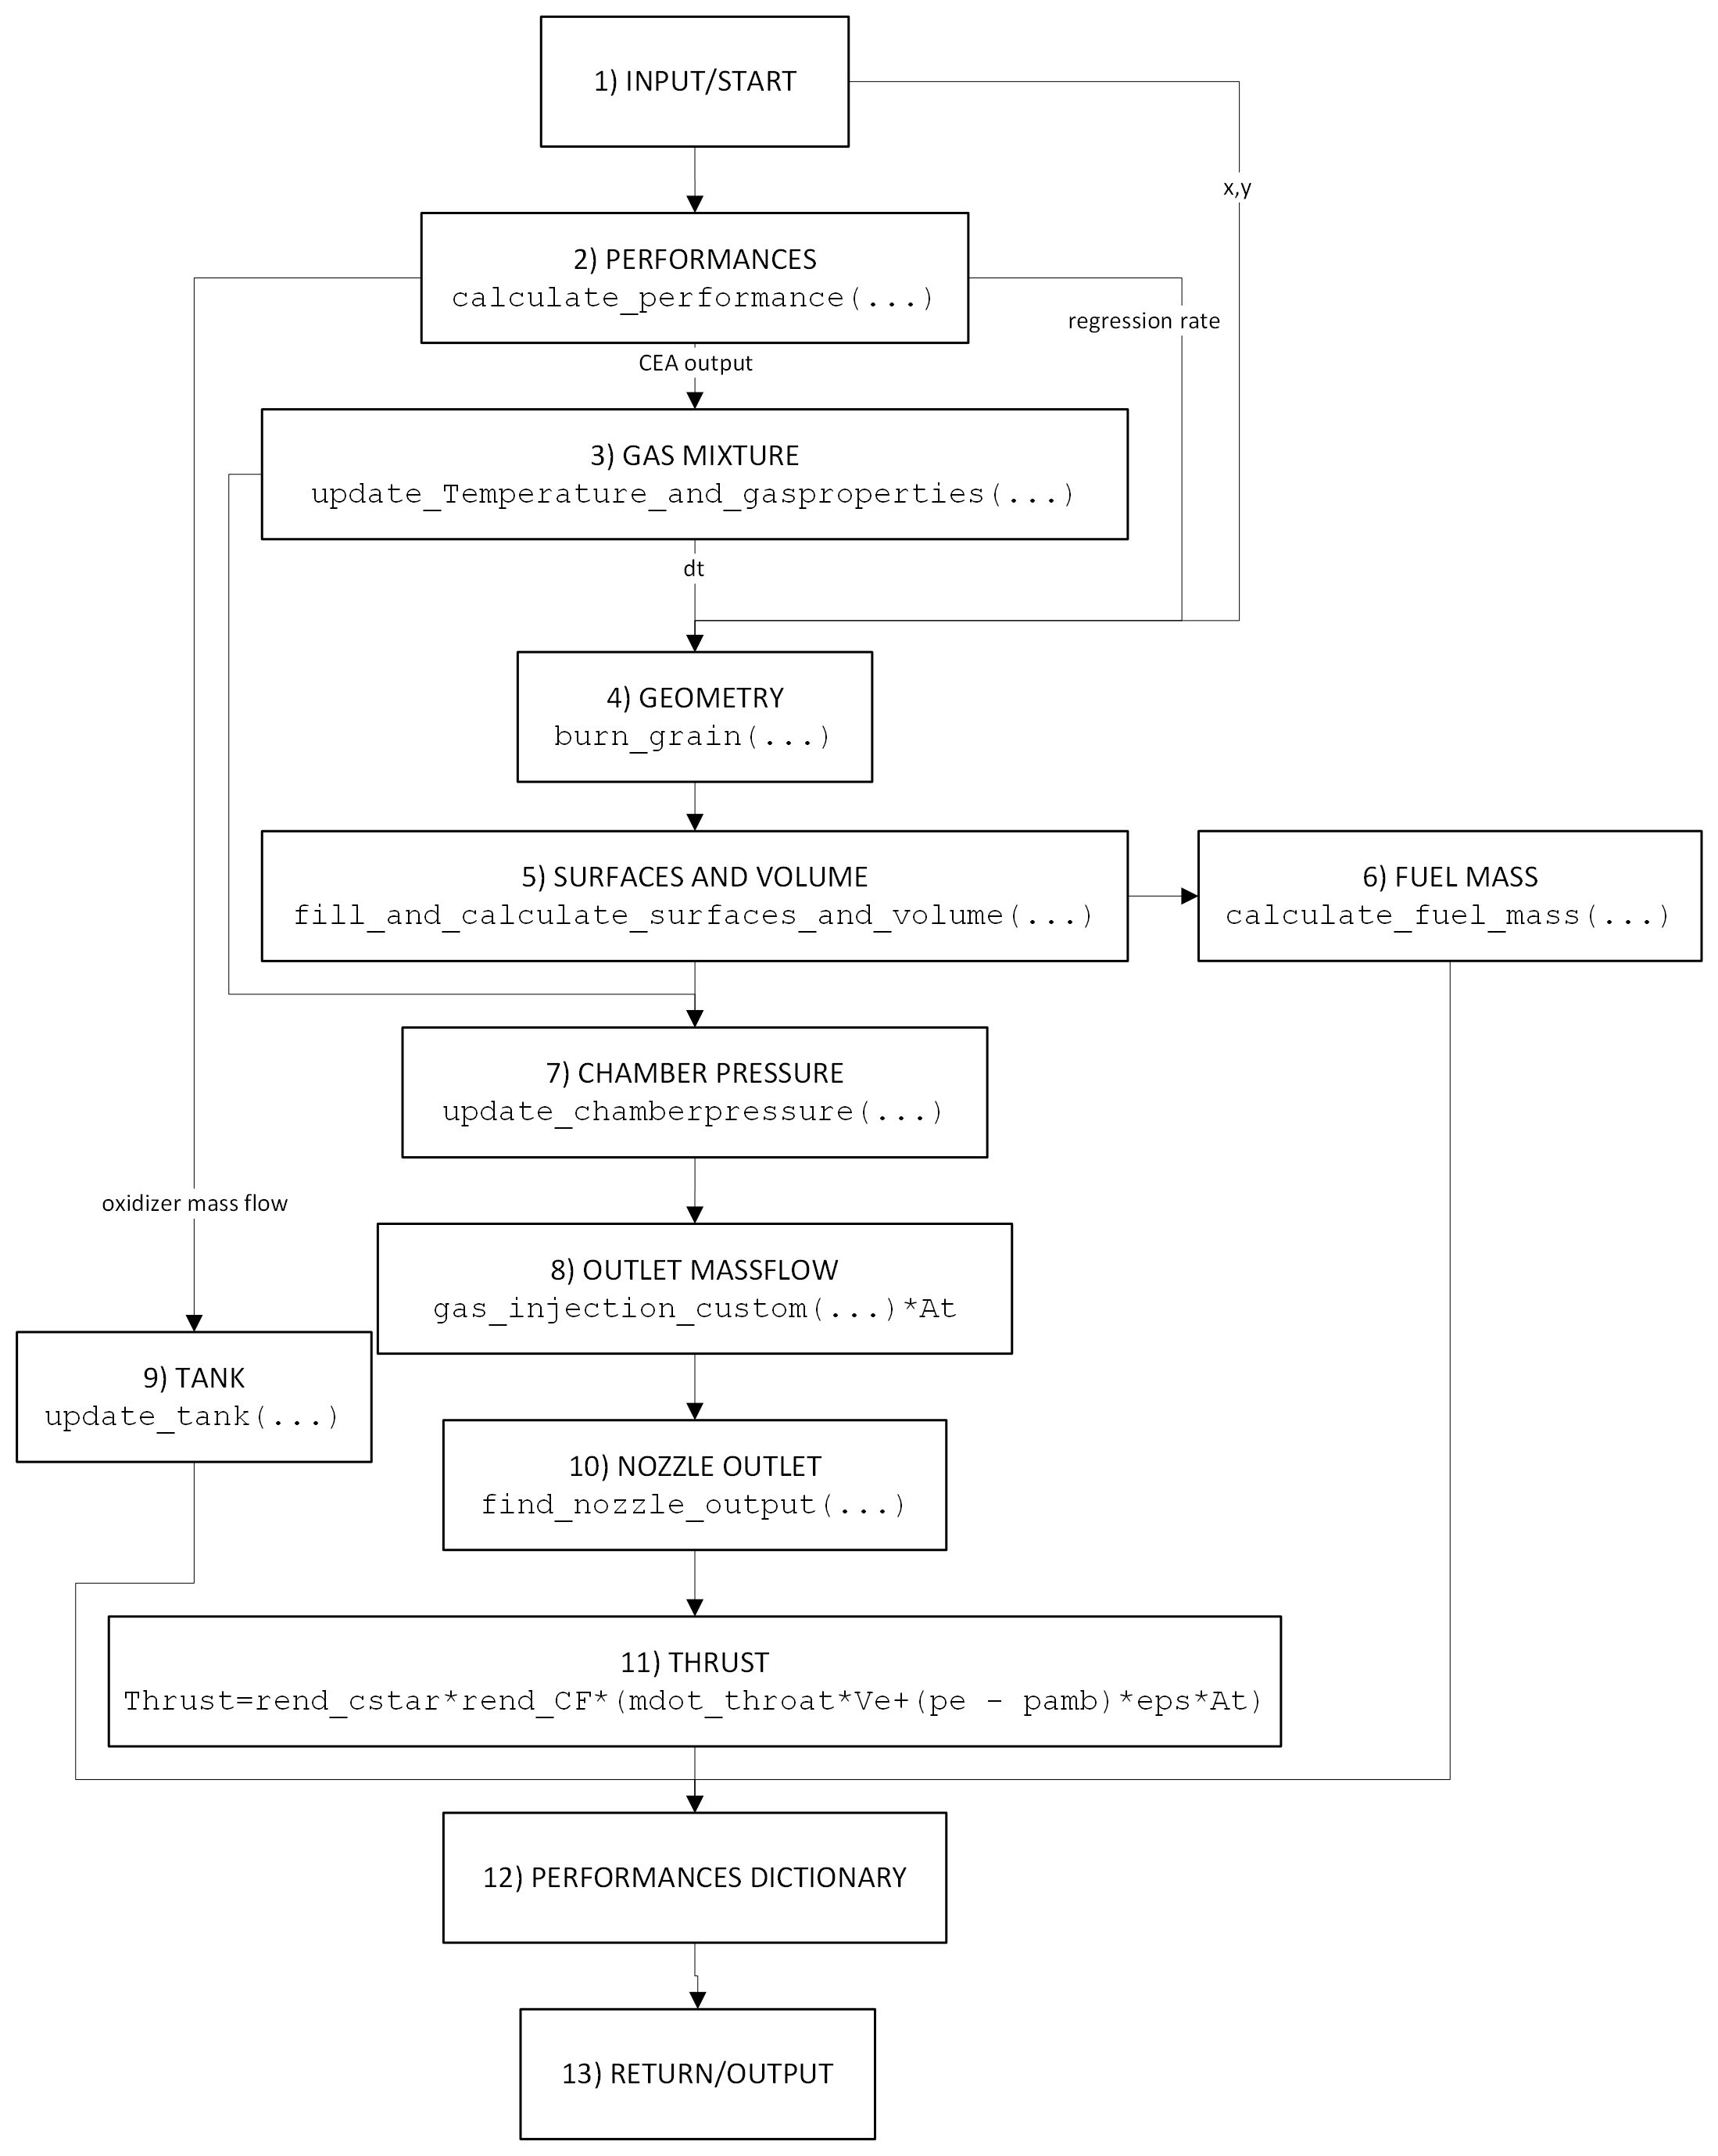
\includegraphics[width=0.9\linewidth]{immagini/burn_flowchart.png}
    \caption{Mission step flowchart}
    \label{fig:flowchartstep}
\end{figure}
The \verb|performances| dictionary is built as in Table \ref{Tab: PerfDicts}.

\begin{table}[h!]
\centering
\resizebox{\textwidth}{!}{
\begin{tabular}{|l|}
\hline
\textbf{Common values}\\
\hline
Chamber pressure "pc" [Pa]\\
Injection pressure "p\_inj" [Pa]\\
Time step "dt" [s]\\
Thrust "Thrust" [N]\\
Oxidizer massflow "mdot\_ox" [kg/s]\\
Fuel massflow "mdot\_fuel" [kg/s]\\
Total inlet massflow "mdot" [kg/s]\\
Total outlet massflow "mdot\_throat" [kg/s]\\
Chamber total temperature "Tc" [K]\\
Molecular weight "MW" [kg/kmol]\\
Specific heat ratio "gamma"\\
Expansion ratio "eps"\\
Grain points x-coordinates "x" [m]\\
Grain points y-coordinates "y" [m]\\
Port area "Ap" [m$^2$]\\
Burning area "Ab" [m$^2$]\\
Chamber internal volume "Vol\_chamber" [m$^3$]\\
Fuel mass "m\_fuel" [kg]\\
Liquid mass in the tank "mL" [kg]\\
Tank pressure "ptank" [Pa]\\
Tank temperature "Ttank" [K]\\
Exit Mach "Me"\\
Exit temperature "Te" [K]\\
Exit pressure "pe" [Pa]\\
Ambient pressure "pamb" [Pa]\\
Entropy dictionary "entropies"\\
Mass dictionary "masses"\\
Pressure dictionary "pressures"\\
Temperature dictionary "temperatures"\\
\hline
\end{tabular}
\begin{tabular}{|l|l|}
\hline
\textbf{No burn} & \textbf{Burn}\\
\hline
& Oxidizer mass flux "Gox" [kg/(m$^2$s)]\\
& Regression rate "r" [m/s]\\
& Mixture ratio "MR"\\
& Chamber temperature from CEA "Tc\_CEA" [K]\\
& Molecular weight from CEA "MW\_CEA" [kg/kmol]\\
& Specific heat ratio from CEA "gamma\_CEA"\\
& Characteristic velocity (c*) "cstar" [m/s]\\
& Thrust coefficient in vacuum "CFvac"\\
& Thrust coefficient "CF"\\
& Specific impulse in vacuum "Ivac" [s]\\
& Specific impulse "Is" [s]\\
& CEA output flag "flag"\\
Burn flag "burn": False & Burn flag "burn": True\\
\hline
\end{tabular}
}
\caption{Performance keys and values for burn and no-burn conditions.}
\label{Tab: PerfDicts}
\end{table}




\chapter{Conclusions}
The presented work is what will lead to the design of an hynrid rocket engine,
but has a lot of limits and needs futher developements.
The main assumptions are:
\begin{itemize}
	\item Chemical equilibrium for combustion
	\item 0-D combustion chamber
	\item Burned gas acts as ideal
\end{itemize}
Future work:
\begin{itemize}
	\item Surpass chemical equilibrium for combustion
	\item Grain matching for a given tank
	\item Multi-port grain
	\item 1-D combustion with losses calculation
	\item Include injector dimensioning using 1-D models
	\item Include nozzle dimensioning with CEA model selecting shifting or frozen equilibrium
\end{itemize}

\input{ReferencesBibliography}
\appendix

% importa tutte le pagine del PDF; mostra il titolo/numero solo nella prima pagina
%\includepdf[pages=1,pagecommand={\chapter{Appendice A: Scheda di sicurezza N2O}\thispagestyle{plain}}, scale=0.78]{Appendici/N2Osafety.pdf}
%\includepdf[pages=2-,pagecommand={}, scale=0.8]{Appendici/N2Osafety.pdf}

%\includepdf[pages=1,pagecommand={\chapter{Appendice B: Scheda di sicurezza N2}\thispagestyle{plain}}, scale=0.78]{Appendici/N2safety.pdf}
%\includepdf[pages=2-,pagecommand={}, scale=0.8]{Appendici/N2safety.pdf}

\end{document}